\chapter{Abordagem Proposta}

De forma geral, a abordagem proposta seguiu as seguintes etapas:
I.	Obter os dados do GAL.
II.	Armazenar os dados obtidos em seu estado bruto.
III.	Identificar as questões a serem respondidas.
IV.	Integrar os dados de forma consistente.
V.	Processar os dados.
VI.	Gerar visualização dos resultados para as questões estabelecidas.

O GAL tem suas funcionalidades limitadas por perfis de acesso, ou seja, na etapa de extração dos dados o pesquisador colaborador (especialista vinculado a FIOCRUZ) obteve somente dados provenientes dos laboratórios dessa instituição. Além disso, o sistema permite somente a exportação dos dados referentes a um período máximo de 3 meses, o que gerou vários arquivos (no formato CSV) que deveriam ser integrados. Cada um dos arquivos refere-se a solicitações ambulatoriais de pessoas suspeitas de terem contraído alguma doença, como zika. No entanto, nestas bases de dados a chave única (chave primária) é o número da solicitação e não um atributo que identifique os pacientes, dessa forma um problema a ser resolvido é a junção dos dados dos pacientes para que nas análises futuras as consultas possam ser respondidas sem duplicatas. Vale ressaltar também que muitas informações não são preenchidas corretamente, como o endereço, telefone, número da carteirinha do SUS e outros dados que poderiam facilitar a identificação dos pacientes.
Na etapa seguinte, foram armazenados 9 arquivos relacionados a zika e outros 9 relacionados a Febre Amarela. Os atributos desses arquivos seguem na \ref{tab1}. Os campos usados para a etapa de integração e processamento (requisição, paciente, data do nascimento, sexo, data dos primeiros sintomas e data da coleta) estão discriminados nas linhas de cor cinza claro. A quantidade de arquivos para cada doença deve-se ao fato da zika ter apresentado um surto entre 2015 e 2017, enquanto a febre amarela apresentou um surto de 2017 até 2018.

\begin{table}
\centering
\caption{Campos dos Arquivos Sobre Zika e Febre Amarela}
\label{tab1}
\begin{tabular}{lll}
\rowcolor[rgb]{0.502,0.502,0.502} ID & Zika                             & Febre Amarela                     \\
\rowcolor[rgb]{0.753,0.753,0.753} 1  & Requisição                       & Requisição                        \\
2                                    & Requisição Correlativo (S/N)     & Requisição Correlativo (S/N)      \\
3                                    & Regional de Cadastro             & Regional de Cadastro              \\
4                                    & Laboratório de Cadastro          & Laboratório de Cadastro           \\
5                                    & CNES Laboratório de Cadastro     & CNES Laboratório de Cadastro      \\
6                                    & Unidade Solicitante              & Unidade Solicitante               \\
7                                    & CNES Unidade Solicitante         & CNES Unidade Solicitante          \\
8                                    & Municipio do Solicitante         & Municipio do Solicitante          \\
9                                    & IBGE Município Solicitante       & IBGE Município Solicitante        \\
10                                   & Estado do Solicitante            & Estado do Solicitante             \\
11                                   & CNS do Profissional de Saúde     & CNS do Profissional de Saúde      \\
12                                   & Nome Profissional de Saúde       & Nome Profissional de Saúde        \\
13                                   & Reg. Conselho/Matrícula          & Reg. Conselho/Matrícula           \\
14                                   & Agravo da Requisição             & Agravo da Requisição              \\
15                                   & Data da Solicitação              & Data da Solicitação               \\
\rowcolor[rgb]{0.753,0.753,0.753} 16 & Data do 1º Sintomas              & Data do 1º Sintomas               \\
17                                   & Finalidade                       & Finalidade                        \\
18                                   & Descrição Finalidade             & Descrição Finalidade              \\
19                                   & Observação                       & Observação                        \\
20                                   & Núm. Notificação Sinan           & Núm. Notificação Sinan            \\
21                                   & Agravo Sinan                     & Agravo Sinan                      \\
22                                   & CID Agravo Sinan                 & CID Agravo Sinan                  \\
23                                   & Data Notificação Sinan           & Data Notificação Sinan            \\
24                                   & Unidade Notificação Sinan        & Unidade Notificação Sinan         \\
25                                   & CNES Unidade Notificação Sinan   & CNES Unidade Notificação Sinan    \\
26                                   & Município Notificação Sinan      & Município Notificação Sinan       \\
27                                   & IBGE Município Notificação SINAN & IBGE Município Notificação SINAN  \\
28                                   & Núm. Notificação Gal             & Núm. Notificação Gal              \\
29                                   & Agravo Gal                       & Agravo Gal                        \\
30                                   & CID Agravo Gal                   & CID Agravo Gal                    \\
31                                   & Data Notificação Gal             & Data Notificação Gal              \\
32                                   & Unidade Notificação Gal          & Unidade Notificação Gal           \\
33                                   & CNES Unidade Notificação Gal     & CNES Unidade Notificação Gal      \\
34                                   & Município Notificação Gal        & Município Notificação Gal         \\
35                                   & IBGE Município Notificação Gal   & IBGE Município Notificação Gal    \\
36                                   & CNS do Paciente                  & CNS do Paciente                   \\
\rowcolor[rgb]{0.753,0.753,0.753} 37 & Paciente                         & Paciente                          \\
\rowcolor[rgb]{0.753,0.753,0.753} 38 & Data de Nascimento               & Data de Nascimento                \\
39                                   & Idade                            & Idade                             \\
40                                   & Tipo Idade                       & Tipo Idade                        \\
\rowcolor[rgb]{0.753,0.753,0.753} 41 & Sexo                             & Sexo                              \\
42                                   & Idade Gestacional                & Idade Gestacional                 \\
43                                   & Nacionalidade                    & Nacionalidade                     \\
44                                   & Raça/Cor                         & Raça/Cor                          \\
45                                   & Etnia                            & Etnia                             \\
46                                   & Tipo Doc. Paciente 1             & Tipo Doc. Paciente 1              \\
47                                   & Documento Paciente 1             & Documento Paciente 1              \\
48                                   & Tipo Doc. Paciente 2             & Tipo Doc. Paciente 2              \\
49                                   & Documento Paciente 2             & Documento Paciente 2              \\
50                                   & Nome da Mãe                      & Nome da Mãe                       \\
51                                   & Endereço                         & Endereço                          \\
52                                   & Bairro                           & Bairro                            \\
53                                   & CEP de Residência                & CEP de Residência                 \\
54                                   & Municipio de Residência          & Municipio de Residência           \\
55                                   & IBGE Município de Residência     & IBGE Município de Residência      \\
56                                   & Estado de Residência             & Estado de Residência              \\
57                                   & País de Residência               & País de Residência                \\
58                                   & Zona                             & Zona                              \\
59                                   & Telefone de Contato              & Telefone de Contato               \\
60                                   & Nome da Pesquisa                 & Nome da Pesquisa                  \\
61                                   & Número Interno                   & Número Interno                    \\
62                                   & Exame                            & Exame                             \\
63                                   & Metodologia                      & Metodologia                       \\
64                                   & Exame Condicionado (S/N)         & Exame Condicionado (S/N)          \\
65                                   & Exame Restrito (S/N)             & Exame Restrito (S/N)              \\
66                                   & Exame Complementar (S/N)         & Exame Complementar (S/N)          \\
67                                   & Exame Correlativo (S/N)          & Exame Correlativo (S/N)           \\
68                                   & Data de Cadastro                 & Data de Cadastro                  \\
69                                   & Material Biológico               & Material Biológico                \\
70                                   & Localização                      & Localização                       \\
71                                   & Material Clínico                 & Material Clínico                  \\
72                                   & Amostra                          & Amostra                           \\
\rowcolor[rgb]{0.753,0.753,0.753} 73 & Data da Coleta                   & Data da Coleta                    \\
74                                   & Hora da Coleta                   & Hora da Coleta                    \\
75                                   & Usou Medicamento                 & Usou Medicamento                  \\
76                                   & Medicamento                      & Medicamento                       \\
77                                   & Data Início Sintomas             & Data Início Sintomas              \\
78                                   & Kit                              & Kit                               \\
79                                   & Fabricante                       & Fabricante                        \\
80                                   & Lote do Kit                      & Lote do Kit                       \\
81                                   & Reteste                          & Reteste                           \\
82                                   & Data do Encaminhamento           & Data do Encaminhamento            \\
83                                   & Data do Recebimento              & Data do Recebimento               \\
84                                   & Data Início do Processamento     & Data Início do Processamento      \\
85                                   & Data do Processamento            & Data do Processamento             \\
86                                   & Laboratório Responsável          & Laboratório Responsável           \\
87                                   & CNES Laboratório responsável     & CNES do Laboratório Responsável   \\
88                                   & Laboratório de Execução          & Data da Liberação                 \\
89                                   & CNES Laboratório de Execução     & Status Exame                      \\
90                                   & Data da Liberação                & 1º Campo Resultado                \\
91                                   & Status Exame                     & 2º Campo Resultado                \\
92                                   & 1º Campo Resultado               & 3º Campo Resultado                \\
93                                   & 2º Campo Resultado               & 4º Campo Resultado                \\
94                                   & 3º Campo Resultado               & 5º Campo Resultado                \\
95                                   & 4º Campo Resultado               & 6º Campo Resultado                \\
96                                   & Caso                             & Observações do Resultado          \\
97                                   & Etapa tratamento                 &                                   \\
98                                   & Tomou vacina                     &                                   \\
99                                   & Data da Última Dose              &                                   \\
100                                  & Vacina                           &                                   \\
101                                  & Tempo                            &                                   \\
102                                  & Período de Tratamento            &                                   \\
103                                  & Motivo                           &                                   \\
104                                  & Diagnóstico                      &                                   \\
\end{tabular}
\end{table}

Junto ao especialista da FIOCRUZ, foram levantadas as seguintes questões:
I.	Taxa de positividade por metodologia, considerando o tempo de coleta.
II.	Taxa de positividade por material, considerando o tempo de coleta.
III.	Relação entre materiais usados e a taxa de positividade por metodologia.
IV.	Relação, quando houver, da taxa de positividade ao ser aplicada mais de uma metodologia, considerando os tempos de coleta.
V.	Média do tempo de coleta para garantir positividade de cada metodologia e outros dados estatísticos como desvios padrão.
Nota: tempo de coleta é uma medida obtida pela diferença entre a data de coleta e a data dos primeiros sintomas.

Para integrar todos os arquivos, utilizamos o Apache Drill, que é um sistema distribuído gratuito e de código aberto, para análise ad-hoc interativa de conjuntos de dados de grande escala. Projetado para lidar com até
petabytes de dados espalhados por milhares de servidores, seu objetivo é responder a consultas ad-hoc em uma latência baixa.
A arquitetura do drill possui basicamente 3 camadas: usuário, processamento e fonte de dados.
A camada de usuário provê acesso aos dados por meio de interfaces (linha de comando, REST, API e drivers JDBC/ODBC). A camada de processamento permite plugar ou extender linguagens de consulta. Na camada dos dados, configura-se  o acesso as fontes de dado, local e/ou clusterizada. Essas fontes podem ser estruturadas, semiestruturadas ou não estruturadas. \cite{hausenblas2013apache}.
Em nosso cenário, os arquivos são textuais no formato CSV, cujo separador de atributos é o caracter ";" com campos fautantes como strings vazias. Além disso, os arquivos foram armazenados localmente. Esses fatores foram configurados em uma interface do próprio Apache Drill, para aceitar corretamente o formato e para endereçar os arquivos por meio do Sistema Padrão de Arquivos (DFS).

As tarefas de manipulação dos dados na etapa de processamento dos dados foi feita na linguagem python por meio da biblioteca \ref{https://pandas.pydata.org/}{Pandas} e o pacote \ref{http://www.numpy.org/}{NumPy}, que juntas são atualmente algumas das ferramentas mais conhecidas e poderosas em data science.
No Pandas, pudemos utilizar a estrutura de dados Dataframe para armazenar o caminho dos arquivos, a chave primária de cada tupla (número da requisição), todas as aparições dos nomes dos pacientes, seu respectivo gênero e data de nascimento. Esses dados foram processados por meio da biblioteca \ref{https://recordlinkage.readthedocs.io/en/latest/index.html}{Record Linkage Toolkit} para deduplicar os registros e identificar cada paciente.
A obtenção dos dados e a subsequente transformação em um Dataframe como descrito anteriormente foi feita por meio da biblioteca \ref{https://pydrill.readthedocs.io/en/latest/}{pydrill}, que é uma abstração para python de comandos a serem enviados ao Apache Drill, facilitando o desenvolvimento.
A identificação de duplicatas foi feita por meio de 3 etapas: limpesa dos dados, indexação e comparação.

O Dataframe resultante das etapas de processamento dos dados contém como atributos: caminho do arquivo para a tupla, chave primária do arquivo (número da requisição), código identificador (substitui as informações dos pacientes mantendo o anonimato) e tempo de coleta para a requisição da respectiva tupla.
Esse Dataframe foi salvo por meio do Apache Drill em uma view permanente.
Dessa forma é possível mapear as solicitações como pacientes únicos, ao aplicar consultas que utilizem a view e os arquivos textuais em seu formato bruto.
O fluxo de trabalho da abordagem como um todo pode ser exemplificado na figura \ref{fig4}. A tarefa de executar consultas do Apache Drill possui um fluxo interno, da própria ferramenta, que é descrito abaixo e mostrado na figura \ref{fig5}.
I. Um cliente do drill faz uma consulta. Um cliente Drill é um driver JDBC, ODBC, interface de linha de comandos ou uma API REST. Qualquer Drillbit (responsável por aceitar consultas vindas de clientes) em um cluster pode aceitar consultas. Não há conceito mestre-escravo.
II. O Drillbit analisa a consulta, otimiza-a e gera um plano de consulta distribuído que é otimizado para uma execução rápida e eficiente.
III. O Drillbit que aceita a consulta torna-se o nó Drillbit da solicitação. Ele obtém uma lista de nós Drillbit disponíveis no cluster do ZooKeeper. O Drillbit de direcionamento determina os nós apropriados para executar vários fragmentos do plano de consulta para maximizar a localidade dos dados.
IV. O Drillbit programa a execução de fragmentos de consulta em nós individuais de acordo com o plano de execução.
V. Os nós individuais concluem sua execução e retornam dados para o Drillbit de acionamento.
VI. Os resultados são encaminhados para o cliente por meio de streams.

\begin{figure}[!ht]
\centering
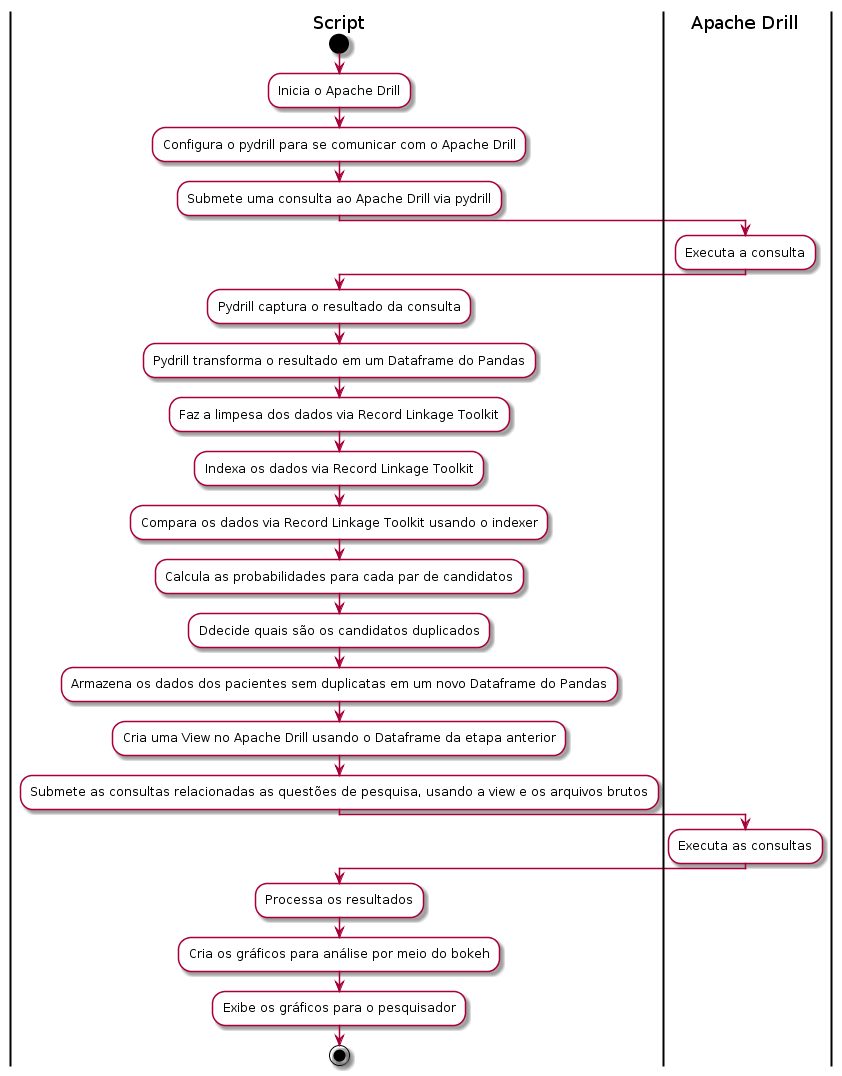
\includegraphics[width=0.3\linewidth]{figuras/wf_script.png}
\caption{Fluxo de trabalho da abordagem proposta}
\label{fig4}
\end{figure}

\begin{figure}[!ht]
\centering
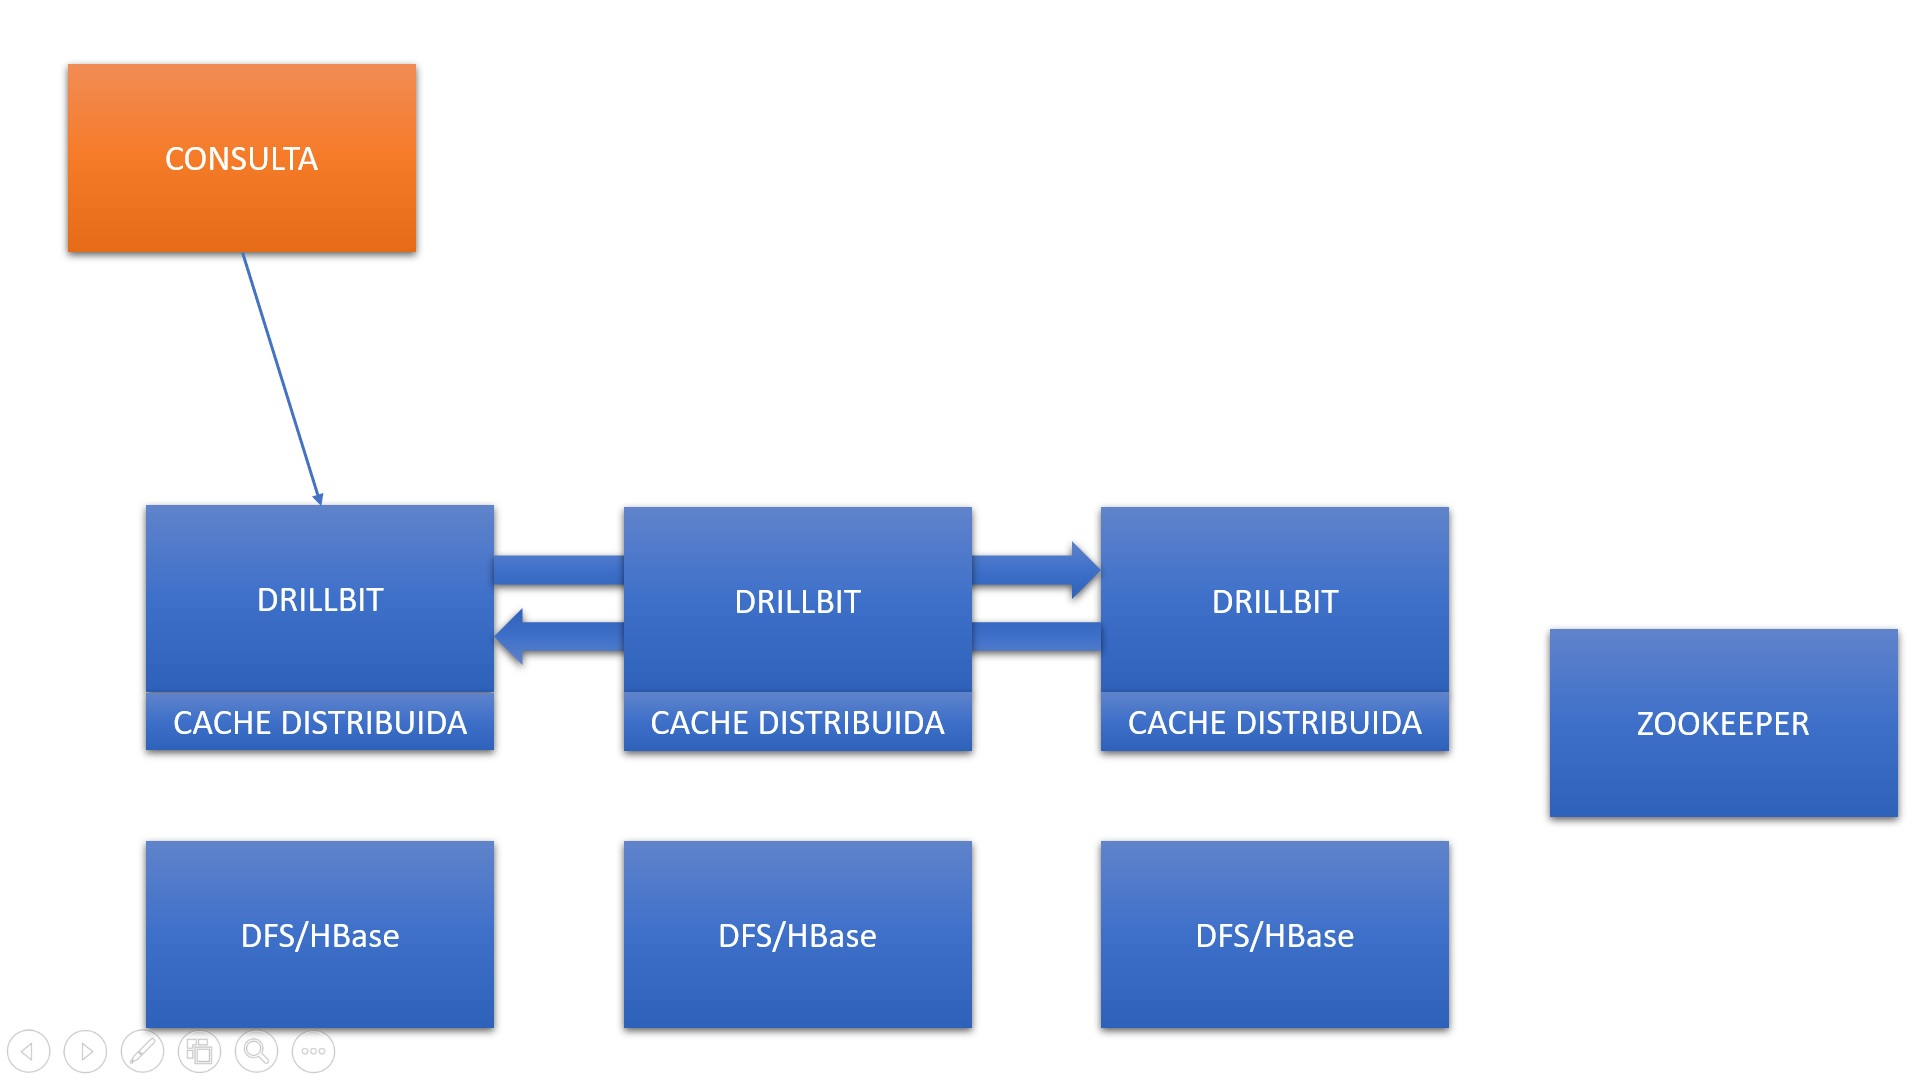
\includegraphics[width=0.3\linewidth]{figuras/wf_drill.jpg}
\caption{Fluxo interno de Consulta do Apache Drill, retirado de: https://drill.apache.org/architecture/}
\label{fig5}
\end{figure}